\documentclass[border=2pt]{standalone}
\usepackage{fontspec}
\setmainfont{Liberation Serif}
\usepackage{tikz,graphicx,pgfplots}
\usetikzlibrary{arrows.meta,positioning,matrix,calc}
\pgfplotsset{compat=1.18}
\definecolor{forest}{HTML}{176044}
\definecolor{sage}{HTML}{EAF4EE}
\definecolor{rulec}{HTML}{CBD4CF}
\definecolor{ink}{HTML}{192723}
\definecolor{warm}{HTML}{F3ECE4}
\tikzset{all/.style={font=\fontsize{10.5pt}{12.5pt}\selectfont,text=ink},
box/.style={all,draw=rulec,fill=sage,rounded corners=2pt,align=center,inner sep=4pt,minimum height=0.9cm},
mutedbox/.style={box,fill=white},warmbox/.style={box,fill=warm},
flow/.style={-{Latex[length=2.4mm]},line width=.65pt,draw=forest}}
\begin{document}
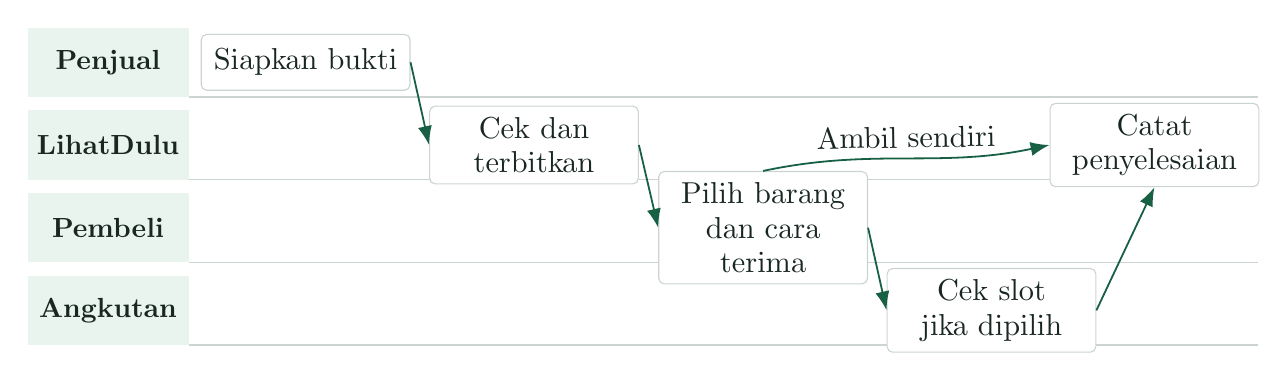
\begin{tikzpicture}[x=1cm,y=1cm]
\foreach \name/\y in {Penjual/0,LihatDulu/-1.05,Pembeli/-2.10,Angkutan/-3.15}{
 \fill[sage] (0,\y+.44) rectangle (2.05,\y-.44);
 \node[all,font=\fontsize{10.3pt}{12pt}\selectfont\bfseries] at (1.02,\y) {\name};
 \draw[rulec] (2.05,\y-.44)--(15.63,\y-.44);
}
\node[mutedbox,text width=2.37cm,minimum height=.71cm] (a) at (3.53,0) {Siapkan bukti};
\node[mutedbox,text width=2.37cm,minimum height=.71cm] (b) at (6.43,-1.05) {Cek dan terbitkan};
\node[mutedbox,text width=2.37cm,minimum height=.71cm] (c) at (9.34,-2.10) {Pilih barang dan cara terima};
\node[mutedbox,text width=2.37cm,minimum height=.71cm] (d) at (12.24,-3.15) {Cek slot jika dipilih};
\node[mutedbox,text width=2.37cm,minimum height=.71cm] (e) at (14.31,-1.05) {Catat penyelesaian};
\draw[flow] (a.east)--(b.west);
\draw[flow] (b.east)--(c.west);
\draw[flow] (c.east)--(d.west);
\draw[flow] (c.north) to[out=12,in=192] node[all,above,sloped]{Ambil sendiri} (e.west);
\draw[flow] (d.east)--(e.south);
\end{tikzpicture}
\end{document}
